%% ==============================
\chapter{Methoden der Dimensionsreduktion}
\label{ch:MethodenDerDimRed}
%% ==============================

Nachdem nun die Motivation und Idee hinter der Dimensionsreduktion in \chapref{ch:Enleitung} und
die mathematische Formulierung in \chapref{ch:Dimensionsreduktion} allgemein angeschaut wurde,
werden nun einige konkrete Methoden der Dimensionsreduktion vorgestellt.

In jüngster Zeit haben vor allem verschiedenste Varianten von neuronale Netzen einen hohen Grad an
Aufmerksamkeit durch bemerkenswerte Errungenschaften in Gebieten der automatischen Spracherkennung
oder \textit{Computer Vision} erlangt. Fraglich ist, ob diese neuen Algorithmen auch auf dem
Bereich der Dimensionsreduktion einen entscheidenden Fortschritt gemacht haben. Deshalb werden die
Algorithmen in dieser Arbeit in \textit{statistischen} und \textit{Machine Learning} Methoden
unterteilt, um diese später in \chapref{ch:Vergleich} gegenüberstellen zu können. Statistische
Methoden haben eine solide theoretische Fundierung und sind meist etablierte Algorithmen auf einem
jeweiligen Gebiet, wie das zum Beispiel mit der Hauptkomponentenanalyse
(\subsecref{ch:MethodenDerDimRed:statistisch:PCA}) der Fall ist. Machine Learning Methoden hingegen
haben lediglich das Ziel, von Trainingsdaten auf neue, das heißt ungesehene (Test-)Daten zu
generalisieren. Neuronale Netze sind hierfür ein Paradebeispiel und werden deshalb in
\secref{ch:MethodenDerDimRed:modern} eingehend behandelt. Allerdings ist hier aus jeder Kategorie
nur eine kleine repräsentative Auswahl getroffen worden. Weitere wichtige Algorithmen, die hier
nicht vorgestellt werden können sind beispielsweise \dots \todo{Aufzählung der Algorithmen die
	nicht betrachtet werden hier oder in der Einleitung?}.

\section{Statistische Methoden}
\label{ch:MethodenDerDimRed:statistisch}

Zu den statistischen Methoden, die in dieser Arbeit vorgestellt werden, gehören die
\newterm{Hauptkomponentenanalyse} (PCA) in \subsecref{ch:MethodenDerDimRed:statistisch:PCA} sowie
die nichtlineare Erweiterung der Hauptkomponentenanalyse, die Kernel PCA
(\subsecref{ch:MethodenDerDimRed:statistisch:kPCA}). Außerdem wird die Multidimensionale Skalierung
(MDS) in \subsecref{ch:MethodenDerDimRed:statistisch:MDS} als Vertreter der statistischen Methoden
genauer behandelt.

%% ==============================
\subsection{Principal Component Analysis}
\label{ch:MethodenDerDimRed:statistisch:PCA}
\nomenclature[Z]{PCA}{Principal Component Analysis}

Principal Component Analysis ist \textit{die} Methode der Dimensionsreduktion und wurde erstmals
von \textcite{Pearson.1901} und \textcite{Hotelling.1933} entwickelt. Trotz des mittlerweile
relativ hohen Alters ist die Hauptkomponentenanalyse immer noch aufgrund der simplen Anwendbarkeit
oft die erste Wahl einer Dimensionsreduktionsmethode. Im Folgenden möchte ich kurz auf die zentrale
Idee und Motivation (\ref{ch:MethodenDerDimRed:statistisch:PCA:Grundidee}) der
Hauptkomponentenanalyse, sowie die mathematische Herleitung der sogenannten
\newterm{Hauptkomponenten} (Unterabschnitte \ref{ch:MethodenDerDimRed:statistisch:PCA:Definition}
und \ref{ch:MethodenDerDimRed:statistisch:PCA:HerleitungPC}) eingehen.

\subsubsection{Grundidee}
\label{ch:MethodenDerDimRed:statistisch:PCA:Grundidee}
Die zentrale Idee der Hauptkomponentenanalyse ist die Transformation des Koordinatensystems in einer möglichst \textit{verlustfreien} Art und Weise. Verlustfrei bedeutet im Kontext der Hauptkomponentenanalyse, dass möglichst viel Variation in den Daten erhalten bleiben soll \parencite[vgl.][1]{Jolliffe.2002}. Möchte man dann die Dimension von $D$ auf die intrinsische
Dimension $d$ reduzieren, so wählt man einfach die \textit{ersten} $d$ Hauptkomponenten.\rewrite{Zu
	ungenau, und hier gleich das Ergebnis zu erwähnen ist auch nicht so hilfreich für die Grundidee}
Was diese Hauptkomponenten sind und wie man sie herleitet, wird im Folgenden genauer betrachtet.

\subsubsection{Definition der Hauptkomponenten}
\label{ch:MethodenDerDimRed:statistisch:PCA:Definition}
Als Ausgangsbasis wird ein $D$-dimensionalen Zufallsvektor $\rvect{x} = \tr{(\rv{x}_1, \ldots, \rv{x}_D)}$ mit $\Exp[\rvect{x}] = \vect{0}$ angenommen und das Ziel ist es, eine $k$-dimensionale Repräsentation $\rvect{y} = \tr{(\rv{y_1},\ldots,\rv{y}_k)}$ zu erhalten. Idealerweise setzt man $k$ auf die intrinsische Dimension $d$ von $\rvect{x}$, hier soll jedoch nur der Fokus auf die allgemeine Dimensionsreduktion gelegt werden. Wir drücken also $\rvect{y}$ als eine Linearkombination des ursprünglichen hochdimensionalen Vektors $\rvect{x}$ wie folgt aus:
\begin{equation}
	\rv{y}_i = \tr{\vect{a}_i} \rvect{x} = a_{i1} \rv{x}_1 + \cdots + a_{iD} \rv{x}_D
	\quad i = 1,\ldots,k
\end{equation}
wobei $\vect{a}_i$ die \newterm{Koeffizienten} (auch: Ladungen) der $i$-ten Hauptkomponente sind \parencite[vgl.][2]{Jolliffe.2002}. Die Anzahl $k$ der Hauptkomponenten bestimmt den Grad der
Dimensionsreduktion, kann jedoch beliebig zwischen $1 \leq k \leq D$ gewählt werden.\footnote{Der
	Grenzfall $k = D$ wird oft für eine Anonymisierung des Datensatzes mit personenbezogenen Daten
	verwendet. Beispielsweise kann so bei Finanztransaktionen der Datensatz mithilfe von PCA
	vorverarbeitet (\textit{Preprocessing}) und erst dann veröffentlicht werden.}

\subsubsection{Herleitung der Hauptkomponenten}
\label{ch:MethodenDerDimRed:statistisch:PCA:HerleitungPC}
Betrachtet wird nun zunächst lediglich die \textit{erste} Hauptkomponente $\tr{\vect{a}_1} \rvect{x}$ und erinnern uns daran, dass wir wie in \subsecref{ch:MethodenDerDimRed:statistisch:PCA:Grundidee} erwähnt möglichst viel Variation von $\rvect{x}$ erhalten möchten. Daher wird die erste Hauptkomponente so gewählt, dass die Varianz maximal wird:
\begin{equation}
	\label{eq:PCA-Optimierungsproblem}
	\max_{\vect{a}_1} \Var \left( \tr{\vect{a}_1} \rvect{x} \right) = \max_{\vect{a}_1} \tr{\vect{a}_1} \mat{\Sigma} \vect{a}_1
\end{equation}
wobei $\mat{\Sigma}$ die Kovarianzmatrix von $\rvect{x}$ ist. Dieses Maximierungsproblem ist jedoch nach oben unbeschränkt, weshalb man zusätzlich die Bedingung
\begin{equation}
	\norm{ \vect{a}_1 }^2 = \tr{\vect{a}_1} \vect{a}_1 = 1
\end{equation}
zum nun \textit{restringierten} Maximierungsproblem hinzufügt, welches mithilfe des Lagrange-Ansatzes gelöst werden kann. Diese Bedingung führt dazu, dass wir eine orthogonale Transformation\unsure{Zitat hinzufügen oder mehr dazu sagen, ein satz reicht nicht} erhalten. Wie sich heraustellt, ist dieses Maximierungsproblem ein Eigenwertproblem und kann somit effizient gelöst werden \parencite[vgl.][4 -- 6]{Jolliffe.2002}\unsure{Vlt hier die Lagrange Gleichung aufstellen und selber
	lösen, um zu sehen, dass man bei einem Eigenwertproblem landet}. Man erhält somit die Koeffizienten
der ersten Hauptkomponente $\vect{a}_1$, welche ein Eigenvektor von $\mat{\Sigma}$ mit zugehörigem
Eigenwert
\begin{equation}
	\lambda_1 = \Var(\tr{\vect{a}_1} \rvect{x})
\end{equation}
sind. Man beachte, dass dies gleichzeitig die Zielfunktion unseres Optimierungsproblems (\eqref{eq:PCA-Optimierungsproblem}) ist. Das bedeutet, dass die Koeffizienten der ersten Hauptkomponente dem Eigenvektor mit dem größten zugehörigen Eigenwert entspricht.

Um nun die zweite Hauptkomponente zu erhalten, wird wieder die Varianz mit der
Einheitsvektor-Nebenbedingung $\norm{\vect{a}_2}$ = 1 maximiert. Zusätzlich muss jedoch gelten,
dass die zweite Hauptkomponente zur Ersten \textit{unkorreliert}\unsure{wieso muss das gelten? Ein
	satz dazu wäre gut} ist \parencite[5]{Jolliffe.2002}, das heißt
\begin{equation}
	\Cov(\tr{\vect{a}_1}\rvect{x}, \tr{\vect{a}_2}\rvect{x}) = 0
\end{equation}
Auch dieses Optimierungsproblem ist ein Eigenwertproblem und man erhält, dass die Koeffizienten $\vect{a}_2$ der zweiten Hauptkomponente der Eigenvektor mit dem zweitgrößten Eigenwert von $\mat{\Sigma}$ ist.
Generell lässt sich zeigen, dass die Koeffizienten der $i$-ten Hauptkomponente dem Eigenvektor mit $i$-ten nach der Größe geordneten Eigenwert entspricht \parencite[6]{Jolliffe.2002}. Aus diesem Grund lassen sich die Hauptkomponenten kompakt durch
\begin{equation}
	\rvect{y} = \tr{\mat{A}} \rvect{x}
\end{equation}
ausdrücken, wobei $\mat{A} = [\vect{a}_1,\ldots,\vect{a}_k] \in \real^{D \times k}$ die Matrix der Eigenvektoren als Spaltenvektoren ist und wieder $1 \leq k \leq D$ gilt.

\subsubsection{Erweiterungen}
\label{ch:MethodenDerDimRed:statistisch:PCA:Erweiterungen}
Trotz der großen Beliebtheit der Hauptkomponentenanalyse hat diese Methode natürlich auch ihre Nachteile, weswegen zahlreiche Erweiterungen wie zum Beispiel \ldots\addref entwickelt wurden.
Ein Schwachpunkt von PCA ist, dass die orthogonale Transformation auf die Eigenvektorbasis der Kovarianzmatrix inhärent linear ist. Die Hauptkomponentenanalyse ist also in dieser klassischen Form nicht in der Lage, eine nichtlineare Mannigfaltigkeit in den Daten zu erkennen. Deswegen wurde unter anderem eine Generalisierung von PCA von \textcite{Scholkopf.1997} entwickelt, die sogenannte \newterm{Kernel Principal Component Analysis} (kPCA). Diese Methode wird in \subsecref{ch:MethodenDerDimRed:statistisch:kPCA} genauer behandelt.

%% ==============================
\subsection{Kernel Principal Component Analysis}
\label{ch:MethodenDerDimRed:statistisch:kPCA}
\nomenclature[Z]{kPCA}{Kernel Principal Component Analysis}
Wie soeben erwähnt ist die Kernel Principal Components Analysis insofern eine Generalisierung der klassischen Hauptkomponentenanalyse, dass auch nichtlineare Zusammenhänge erkannt werden können.
Um das zu erreichen, bedient man sich am sogenannten \newterm{Kernel Trick}, der beispielsweise erfolgreich auf \textit{Support Vector Machines} \parencite{Boser.1992} angewandt wurde. Dazu gehen wir wieder in
\subsecref{ch:MethodenDerDimRed:statistisch:kPCA:Grundidee} auf die Grundidee dieser Methode ein
und befassen uns dann in \subsecref{ch:MethodenDerDimRed:statistisch:kPCA:AnwendungKernelTrick}
kurz mit der konkreten Vorgehensweise bei der Kernel PCA.

\subsubsection{Grundidee}
\label{ch:MethodenDerDimRed:statistisch:kPCA:Grundidee}

Die Grundidee der Kernel PCA ist es, die Daten mithilfe einer Abbildung $\bm{\phi}$ in einen Raum
$\mathcal{H}$ abzubilden, der nichtlinear mit dem Ursprungsraum \unsure{vlt hier einfach $\real^D$
	anstelle von $\mathcal{X}$ benutzen um Verwirrung zu vermeiden. Vlt muss ich dafür auch die
	Begriffe eindeutiger definieren (feature space und input space)} $\mathcal{X}$ von $\rvect{x}$
verbunden ist. Der Raum $\mathcal{H}$ wird in diesem Kontext auch Merkmalsraum (engl.
\textit{feature space}) genannt und kann potentiell sehr hochdimensional sein. Die Motivation
dahinter ist, dass die Daten in $\mathcal{X}$ auf einer \textit{nichtlinearen} Mannigfaltigkeit
liegen können, während sie in $\mathcal{H}$ auf einer \textit{linearen} Mannigfaltigkeit liegen und
damit für lineare Dimensionsreduktionsmethoden wie PCA geeignet sind. Nach der Transformation wird
also die lineare Hauptkomponentenanalyse durchgeführt, um damit die niedrigdimensionale
Repräsentation $\rvect{y}$ zu erhalten. Der entscheidene Punkt ist jedoch, dass man diesen
\enquote{Umweg} über die Abbildung $\bm{\phi}$ nicht konkret berechnen muss, sondern mithilfe einer
Kernel-Funktion $\kappa: \mathcal{X} \times \mathcal{X} \rightarrow \real$ implizit miteinbeziehen
kann \parencites[586 -- 588]{Bishop.2006}[583]{Scholkopf.1997}. Dies ist die Eleganz der Kernel-Methoden wie
Kernel PCA und daher kommt auch die Bezeichnung \textit{Kernel Trick}.\missingfigure{hier könnte
	eine bildliche Beschreibung sehr gut passen}

Für eine eingehendere Behandlung des Kernel Tricks und anderer Kernel-Methoden wird auf
\textcite{ShaweTaylor.2011} verwiesen.

\subsubsection{Anwendung des Kernel Tricks}
\label{ch:MethodenDerDimRed:statistisch:kPCA:AnwendungKernelTrick}

Die Kernel-Funktion ist definiert als das Skalarprodukt im transformierten Raum \parencite[60]{ShaweTaylor.2011}:
\begin{equation}
	\kappa(\vect{x}_i, \vect{x}_j) = \tr{\bm{\phi}(\vect{x}_i)} \bm{\phi}(\vect{x}_j)
\end{equation}
Damit man den Kernel Trick anwenden kann, muss die Hauptkomponentenanalyse in eine Form gebracht werden, in der nur Skalarprodukte von $\rvect{x}$ vorkommen. Dann können alle Skalarprodukte durch die Kernel-Funktion ersetzt werden \parencite[586]{Bishop.2006} und man umgeht die explizite Berechnung von $\bm{\phi}$.

Man berechnet also die $n \times n$ \textit{Kernel Matrix}
\begin{equation}
	\mat{K}_{ij} = \kappa(\vect{x}_i, \vect{x}_j) \qquad \text{für}\; i,j = 1,\ldots,n
\end{equation}
welche anschließend zentriert werden muss \parencite[598]{Bishop.2006}. Nun können die Eigenvektoren und Eigenwerte von $\mat{K}$ bestimmt und
damit die Projektion auf die niedrigdimensionale Repräsentation $\rvect{y}$ berechnet
werden.\rewrite{Diesen Abschnitt (3.1.2.2) muss ich nochmal ganz umschreiben}

%% ==============================
\subsection{Multidimensionale Skalierung}
\label{ch:MethodenDerDimRed:statistisch:MDS}
\nomenclature[Z]{MDS}{Multidimensionale Skalierung}

\subsubsection{Grundidee}

\newpage

%% ==============================
%% ==============================
\section{Machine Learning Methoden}
\label{ch:MethodenDerDimRed:modern}
%% ==============================
Nachdem in \secref{ch:MethodenDerDimRed:statistisch} einige statistischen Methoden der
Dimensionsreduktion näher betrachtet wurden, werden nun zwei ausgewählte Machine Learning Methoden,
nämlich der \newterm{Autoencoder} in seiner klassischen Form
(\subsecref{ch:MethodenDerDimRed:ML:AE}) sowie der \newterm{Contractive Autoencoder} (CAE)
(\subsecref{ch:MethodenDerDimRed:ML:CAE}) vorgestellt.

Die Bezeichnung der Algorithmen als \enquote{modern} ist hier etwas irreführend, da die
vorgestellten Methoden keineswegs brandneu sind, sich jedoch von\rewrite{Das war noch zum alten
	Titel, muss man umschreiben} der Funktionsweise von den eben vorgestellten statistisch Methoden
abheben. Alle drei Algorithmen sind im Prinzip Varianten von neuronalen Netzwerken -- ein Modell
das in jüngster Zeit für sehr gute Ergebnisse in vielen Gebieten gesorgt hat. Allerdings eilt die
empirische Forschung den neuronalen Netzwerken voraus, da man theoretisch bisher nicht beweisen
konnte, wieso diese Architektur funktioniert. Man stellt lediglich fest, dass je größer das
Netzwerk ist und je mehr Rechenkapazität man zur Verfügung hat, desto besser ist das Ergebnis eines
neuronalen Netzwerkes\addref. Inwiefern dies auf das Gebiet der Dimensionsreduktion zutrifft,
werden wir später in \chapref{ch:Vergleich} sehen.

\subsection{Autoencoder}
\label{ch:MethodenDerDimRed:ML:AE}
\nomenclature[Z]{AE}{Autoencoder}

Der Autoencoder ist ein neuronales Netzwerk, das die Rekonstruktion des Inputvektors $\vect{x}$ aus
den Trainingsdaten lernt. Um das sinnvoll zu erreichen, besitzt der Autoencoder eine bestimmte
Architektur. In der klassischen Form hat das Netzwerk eine ungerade Anzahl an Schichten, sodass in
der Mitte eine \newterm{Bottleneck}-Schicht entsteht \parencite[2]{Bank.2020}. Diese wird als \textit{Bottleneck} bezeichnet, da diese Schicht nur $d < D$
Neuronen besitzt. In diesem Fall wird der Autoencoder als \newterm{unterbestimmt} (engl.
\textit{undercomplete}) bezeichnet \parencite[503]{Goodfellow.2016}.\footnote{Es gibt demnach auch überbestimmte Autoencoder mit $k > D$
	Neuronen in der mittleren Schicht. Diese Variante reduziert die Dimension nicht, sondern erhöht sie \parencite[504]{Goodfellow.2016}.} Damit erzielt die Bottleneck-Schicht die gewünschte
Dimensionsreduktion des Inputvektors, da der Autoencoder lernen muss, den Inputvektor aus dieser
niedrigdimensionalen Repräsentation möglichst verlustfrei zu rekonstruieren \parencites[502]{Goodfellow.2016}[2]{Bank.2020}. \figref{fig:5-layer-Autoencoder} zeigt eine
beispielhafte Architektur eines Autoencoders mit fünf Schichten und dreidimensionalem Bottleneck.
Nehmen wir nun wieder an, dass wir einen $D$-dimensionalen Inputvektor $\rvect{x}$ haben (in diesem
Beispiel ist $D = 12$), dann muss der Autoencoder lernen, $\rvect{x}$ zu kodieren, wobei in der
Mitte des Autoencoders die niedrigdimensionale Repräsentation $\rvect{y}$ gelernt wird. In
\figref{fig:5-layer-Autoencoder} ist $d = 3$. Dies bedeutet, dass durch den Autoencoder eine um den
Faktor 4 reduzierte niedrigdimensionale Repräsentation gelernt werden soll.

Die Nichtlinearität eines Autoencoders wird durch die Auswahl der Aktivierungsfunktionen bestimmt.
Werden ausschließlich lineare Funktionen verwendet, bekommt man einen linearen Autoencoder, welcher
sehr ähnlich zur Hauptkomponentenanalyse ist. Dies wird in
\subsecref{ch:MethodenDerDimRed:ML:AE:VerhaeltnisPCA} noch genauer betrachtet. In den meisten
Fällen werden jedoch \textit{Sigmoid}-Aktivierungsfunktionen eingesetzt, um die Flexibilität der
Architektur auszunutzen \parencite[4]{Charte.2018}.

\begin{figure}[h]
	\label{fig:5-layer-Autoencoder}
	\begin{center}
		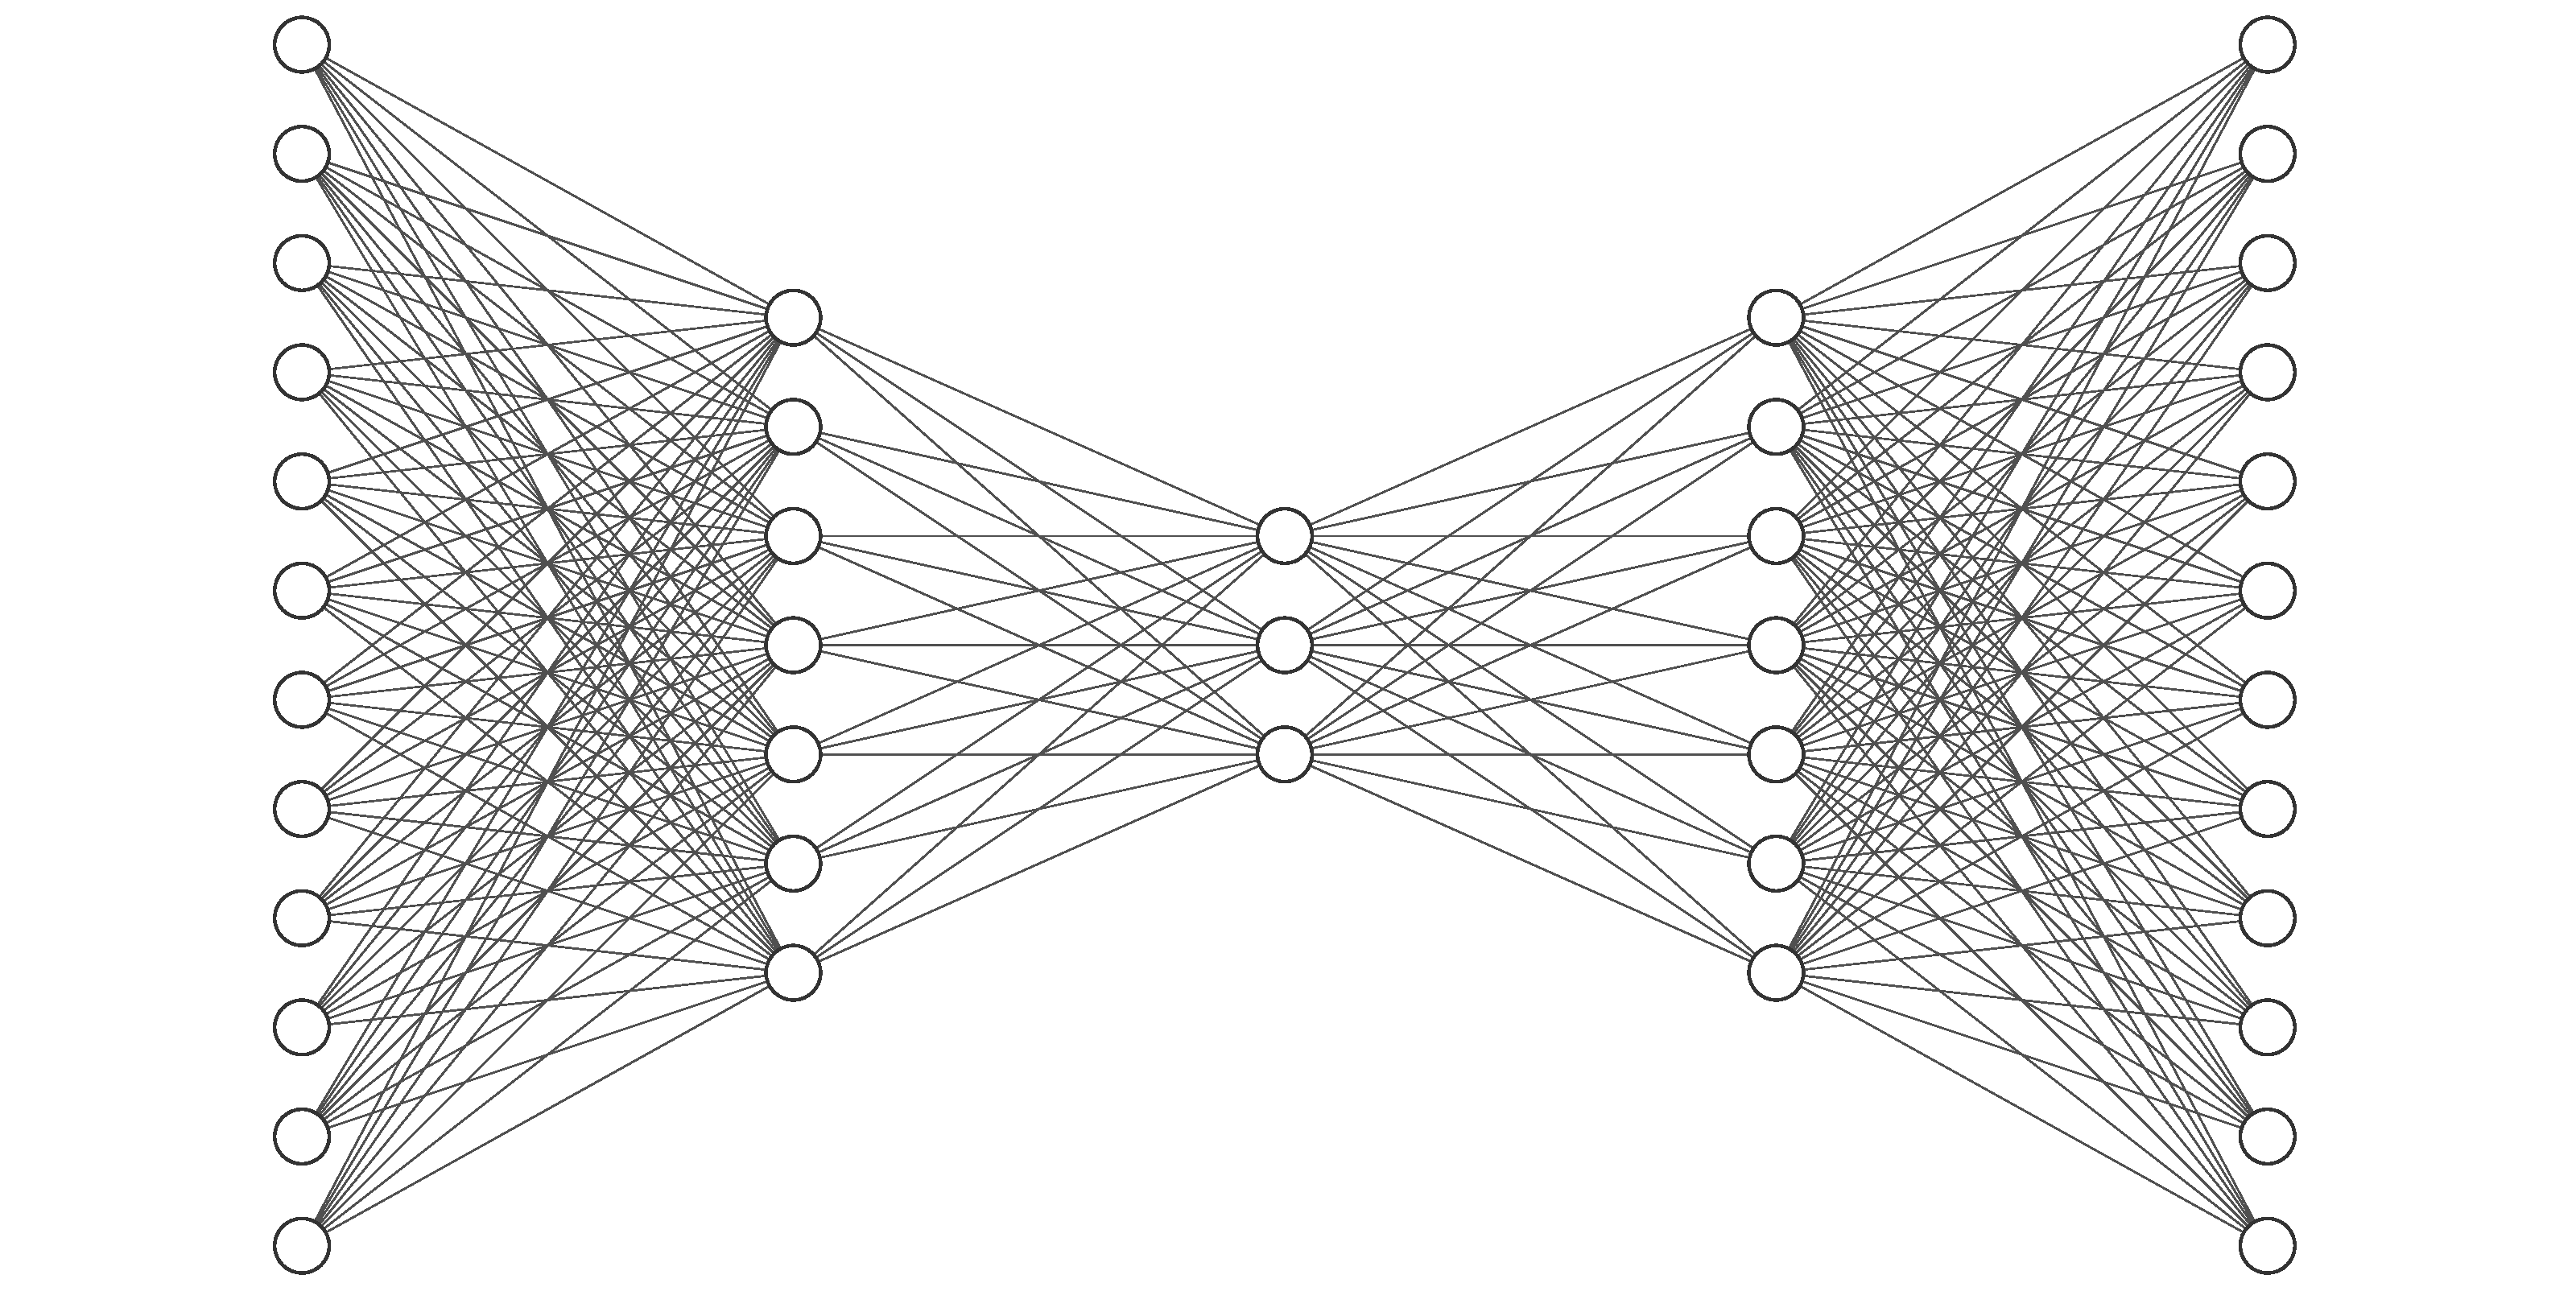
\includegraphics[width=\textwidth]{5_layer_AE.pdf}
		\caption[Schematische Abbildung der Architektur eines Autoencoders]{Gezeigt ist eine schematische Abbildung der Architektur eines (\textit{vollvernetzten}) Autoencoders. Dieser Autoencoder besitzt fünf Schichten, wobei das \textit{Bottleneck} dreidimensional und die \textit{Input}-Dimension zwölf ist. Das bedeutet, dass ein 12-dimensionaler Inputvektor in der Mitte des Autoencoders durch einen dreidimensionalen Vektor kodiert und anschließend wieder dekodiert werden muss, um zu einer möglichst verlustfreien Rekonstruktion zu gelangen. Eigene Darstellung, erstellt mittels \href{https://alexlenail.me/NN-SVG/}{NN-SVG}}
	\end{center}
\end{figure}

\subsubsection{Mathematische Formulierung}
\label{ch:MethodenDerDimRed:ML:AE:MathematischeFormulierung}
Mathematisch gesehen versucht der Autoencoder zwei Funktionen zu lernen. Zum einen den sogenannten \newterm{Encoder} $f: \real^D \rightarrow \real^d$, der den Inputvektor in die niedrigdimensionale Repräsentation $\rvect{y} = f(\rvect{x})$ codiert und zum anderen den \newterm{Decoder} $g: \real^d \rightarrow \real^D$, der diese Repräsentation wieder in den Inputvektor dekodiert. Das Ziel des Autoencoders ist es, den Inputvektor zu rekonstruieren und dabei eine sinnvolle Repräsentation im Bottleneck zu lernen:
\begin{equation}
	\estNormal{\rvect{x}} = g(f(\rvect{x})) \approx \rvect{x}
\end{equation}
wobei $\estNormal{\vect{x}}$ die Rekontruktion des Autoencoders bezeichnet.
Dazu minimiert der Autoencoder eine Fehlerfunktion $L(\vect{x}, \vect{\estNormal{x}})$ die eine große Ungleichheit zwischen dem Input- und Outputvektor bestraft. Hier wird traditionell der mittlere quadratische Fehler (MSE) verwendet, das heißt
\begin{equation}
	L(\vect{x}, \vect{\estNormal{x}}) = \Exp \left[ L_{\text{rec}} \right] = \Exp \left[ \norm{\vect{x} - \vect{\estNormal{x}}}^2 \right]
\end{equation}\unsure{wie definieren? über Erwartungswert?}
\parencite[507]{Goodfellow.2016}, wobei $L_{\text{rec}}$ den Rekonstruktionsfehler bezeichnet. Dieser
Rekonstruktionsfehler ist also lediglich die L2-Norm der Abweichung der beiden Vektoren.

Die Gefahr dabei ist jedoch, dass der Autoencoder bei zu großer Kapazität einfach die
Identitätsfunktion ohne sinnvolle Repräsentation lernt. Dies ist zum Beispiel der Fall, wenn zu
viele Schichten eingesetzt werden und der Autoencoder einfach die Inputvektoren auf Indizes
abbildet. Aus diesem Grund muss ein Autoencoder oftmals regularisiert werden, worauf im nächsten
Unterabschnitt eingegangen wird.

\subsubsection{Regularisierung}
\label{ch:MethodenDerDimRed:ML:AE:Regularisierung}
Um eine sinnvolle Repräsentation $\rvect{y}$ zu erhalten, muss der Autoencoder oftmals
regularisiert, das heißt eingeschränkt, werden. Ein erstes Beispiel hierfür ist der in
\figref{fig:5-layer-Autoencoder} gezeigte unterbestimmte Autoencoder, mit dem eine $d$-dimensionale
Repräsentation in der Mitte forciert wird. Besitzt der Autoencoder jedoch eine zu große Kapazität,
das heißt es werden zu viele Schichten eingesetzt, dann kann der Autoencoder trotz des Bottlenecks
eine uninformative niedrigdimensionale Repräsentation lernen, auch wenn das Bottleneck nur
eindimensional ist. Neben dieser \textit{impliziten} Regularisierung, gibt es deswegen noch einige
weitere explizite Regularisierungsmethoden, die zusätzlich zum Rekonstruktionfehler $L_{rec}$ einen
Bestrafungsterm $\Omega$ zur Fehlerfunktion $L$ hinzufügen.

Eine Umsetzung dessen ist zum Beispiel der \newterm{Sparse Autoencoder}, der eine dünn besetzte
(engl. \textit{sparse}) Repräsentation $\vect{y}$ erzwingt, das heißt nur wenige Einträge von
$\vect{y}$ sind ungleich Null. Dazu wird ein Bestrafungsterm auf den Output des Encoders $\vect{y}
	= f(\vect{x})$ zur Fehlerfunktion hinzugefügt, das heißt
\begin{equation}
	L(\vect{x}, \vect{\estNormal{x}}) = L_{rec} + \Omega(\vect{y})
\end{equation} \Parencite[505]{Goodfellow.2016}. Für das Lernen von Mannigfaltigkeiten besonders interessant ist der
\newterm{Contractive Autoencoder} \parencite{Rifai.2011} , der im \subsecref{ch:MethodenDerDimRed:ML:CAE} genauer behandelt wird.

\subsubsection{Verhältnis zur Hauptkomponentenanalyse}
\label{ch:MethodenDerDimRed:ML:AE:VerhaeltnisPCA}

\textcite{Plaut.2018} haben gezeigt, dass die Repräsentation $\rvect{y}$ eines linearen Autoencoders äquivalent, aber nicht identisch, zu den Hauptkomponenten einer PCA (siehe \secref{ch:MethodenDerDimRed:statistisch:PCA}) ist. Betrachtet man beispielsweise einen einfachen linearen Autoencoder mit drei Schichten, kann der Encoder als
\begin{equation}
	f(\vect{x}) = \mat{W}_1 \vect{x} + \vect{b}_1 = \vect{y}
\end{equation}
und der Decoder als
\begin{equation}
	g(\vect{y}) = \mat{W}_2 \vect{y} + \vect{b}_2 = \estNormal{\vect{x}}
\end{equation}
formuliert werden, wobei $\mat{W}_i$ die Gewichtsmatrizen und $\vect{b}_i$ die Bias-Vektoren des Autoencoders sind ($i = 1, 2$).\footnote{Es kann jedoch gezeigt werden, dass ein Autoencoder mit dieser Architektur und \textit{nichtlinearen} Aktivierungsfunktionen trotzdem eine äquivalente Lösung zur PCA liefert. Für Autoencoder mit mehr als drei Schichten gilt dies nicht mehr.}

\subsection{Contractive Autoencoder}
\label{ch:MethodenDerDimRed:ML:CAE}
\nomenclature[Z]{CAE}{Contractive Autoencoder}